\subsection{LSQ}\label{sec:lsq}

LSQ (load-store queue) keeps loads and stores.
It executes loads out of order and speculatively and keep tracks of violations of memory orderings.

Loads and stores are kept in separate queues, i.e., LQ and SQ.
LQ contains loads and load-reserves.
SQ contains stores, store-conditionals, atomic read-modify-writes, and \emph{fence instructions}.
In future, we should move Reconcile fences to LQ.

In order to observe the memory dependency between loads and stores, each load in LQ keeps track of the index of the immediately preceding SQ entry.
In case a load has been issued from LQ, the load needs to track whether its value will come from the cache or by forwarding from an SQ entry or an SB entry.
When a load tries to issue, it may not be able to proceed because of fences or partially overlapped older stores.
In such cases, the load records the source that stalls it, and retries after the source of the stall has been resolved.
In case of ROB flush, if a load, which is waiting for the memory response, is killed, then this load entry is marked as waiting for a wrong path response.
Because of this bit, we can reallocate this entry to a new load, but not issue it until the bit is cleared.

Atomic instructions (load-reserve, store-conditional and read-modify-write), MMIO accesses, and fence instructions are handled in a conservative way.
When such an instruction reaches the commit slot of the ROB, it is dequeued from LSQ and then executed.
After the execution finishes, the instruction can be committed from ROB.

We try to dequeue LQ as soon as possible to recycle this critical resource.
Dequeuing a load requires all older SQ entries cannot kill the load.
To check this, we sequentially \emph{verify} each SQ entry (from old to young) to make sure the SQ entry cannot squash a younger load.

\subsubsection{Interface}

\begin{figure}
\begin{lstlisting}[caption={}]
typedef struct {
  InstTag            instTag;
  LdQMemFunc         memFunc;
  Bool               unsignedLd;
  ByteEn             byteEn;
  Bool               acq;
  Bool               rel;
  Maybe#(PhyDst)     dst;
  Addr               paddr;
  Bool               isMMIO;
  ByteEn             shiftedBE;
  Maybe#(Exception)  fault;
  Bool               computed;
  Bool               inIssueQ;
  Bool               executing;
  Bool               done;
  Maybe#(LdKilledBy) killed;
  Maybe#(StQTag)     olderSt;
  Bool               olderStVerified;
  Maybe#(StQTag)     readFrom;
  Maybe#(LdQTag)     depLdQDeq;
  Maybe#(StQTag)     depStQDeq;
`ifndef TSO_MM
  Maybe#(LdQTag)     depLdEx;
  Maybe#(SBIndex)    depSBDeq;
`endif
  SpecBits           specBits;
  Bool               atCommit;
  Bool               waitWPResp;
} LdQEntry deriving (Bits, Eq, FShow);
\end{lstlisting}
\caption{Fields in a LQ entry}\label{fig:lq-entry}
\end{figure}

Figure~\ref{fig:lq-entry} shows the fields of a LQ entry:
\begin{itemize}
    \item Field \code{instTag}: is the ROB index of the load.
    \item Field \code{memFunc}: specifies the type of the load (i.e., load or load-reserve).
    \item Field \code{unsignedLd}: indicates if the load is unsigned or not.
    \item Field \code{byteEn}: is a bit mask that specifies the position of the useful load-data bytes in an 8B double-word.
    This bit mask is taken directly from the decode result, and is not shifted according to the address.
    For example, if the load is a load-byte, then the least significant bit of the bit mask is set regardless of the load address.
    \item Field \code{acq}: is true if the entry is a load-reserve and carries a Reconcile fence.
    \item Field \code{rel}: is true if the entry is a load-reserve and carries a Commit fence.
    \item Field \code{dst}: is the destination physical register of the load.
    \item Field \code{paddr}: is the physical address of the load.
    This field is meaningful only if field \code{computed} is true.
    \item Field \code{isMMIO}: indicates if the load is accessing MMIO region.
    This field is meaningful only if field \code{computed} is true.
    \item Field \code{shiftedBE}: specifies the position of the useful load data in an 8B double-word which is loaded from an 8B aligned address.
    This is, it is \code{byteEn} shifted according to the lower bits of the address.
    \item Field \code{fault}: records the exception happened during address translation or MMIO access.
    \item Field \code{computed}: is set true when the translated address is filled into the LQ entry.
    \item Field \code{inIssueQ}: is set true when the load is identified as able to issue (to memory or get bypass), and is unset when the load is truly issued to execution.
    \item Field \code{executing}: is set when the load is issued to execution.
    \item Field \code{done}: is set when the load result returns.
    \item Field \code{killed}: is set when the load is detected to violate memory ordering (e.g., store-to-load dependency or memory consistency).
    The load is not dropped immediately, and will be handled in a way similar to exceptions.
    The reason for the violation is also recorded for performance evaluation.
    \item Field \code{olderSt}: is the SQ index of the immediately older store than this load.
    This field is \code{Invalid} if there is no older stores in SQ.
    \item Field \code{olderStVerified}: is set true to indicate that the load can be retired from LQ, i.e., older entries in SQ should not affect the load.
    This is set by an internal rule of the module.
    \item Field \code{readFrom}: records the source of the load result when the load starts execution.
    This field is meaningful only if field \code{executing} is true.
    \item Field \code{depLdQDeq}: is valid if the load is stalled by an older load-reserve which carries a Reconcile fence.
    This field records the LQ index of the older load.
    This will be reset when the older load is dequeued from LQ.
    \item Field \code{depStQDeq}: is valid if the load is stalled by an older store or fence in SQ.
    This field records the SQ index of the older store or fence.
    This will be reset when the older store or fence is dequeued from SQ.
    \item Field \code{depLdEx}: is valid if the load is stalled by an older load for the same address.
    This field records the LQ index of the older load.
    This will be reset when the older load starts execution.
    \item Field \code{depSBDeq}: is valid if the load is stalled by an entry in store buffer (SB) because of partially overlapped address.
    This field records the index in SB.
    This will be reset when the SB entry is removed.
    \item Field \code{specBits}: is the speculation bit mask.
    \item Field \code{atCommit}: is true when the load has reached the commit slot in ROB.
    \item Field \code{waitWPResp}: is true if this LQ entry is waiting for a wrong-path response, and the current load in this entry cannot start execution.
    This bit will be reset when the wrong-path response returns.
\end{itemize}

\begin{figure}
\begin{lstlisting}[caption={}]
typedef struct {
  InstTag           instTag;
  StQMemFunc        memFunc;
  AmoFunc           amoFunc;
  Bool              byteEn;
  Bool              acq;
  Bool              rel;
  Maybe#(PhyDst)    dst;
  Addr              paddr;
  Bool              isMMIO;
  ByteEn            shiftedBE;
  Data              stData;
  Maybe#(Exception) fault;
  Bool              computed;
  Bool              verified;
  SpecBits          specBits;
  Bool              atCommit;
} StQEntry deriving(Bits, Eq, FShow);
\end{lstlisting}
\caption{Fields in a SQ entry}\label{fig:sq-entry}
\end{figure}

Figure~\ref{fig:sq-entry} shows the fields of a SQ entry:
\begin{itemize}
    \item Field \code{instTag}: is the ROB index of the instruction.
    \item Field \code{memFunc}: specifies the type of the instruction (i.e., store, or store-conditional, or atomic read-modify-write, or fence).
    \item Field \code{amoFunc}: specifies the type of the atomic read-modify-write operation if the instruction is an atomic read-modify-write.
    \item Field \code{byteEn}: is a bit mask that specifies the position of the useful store-data bytes in the 8B double-word in the source register.
    This bit mask is taken directly from the decode result, and is not shifted according to the address.
    For example, if the store is a store-byte, then the least significant bit of the bit mask is set regardless of the store address.
    \item Field \code{acq}: is true if the instruction carries a Reconcile fence (the instruction cannot be a normal store in this case).
    \item Field \code{rel}: is true if the instructoin carries a Commit fence (the instruction cannot be a normal store in this case).
    \item Field \code{dst}: is the destination physical register of the load.
    \item Field \code{paddr}: is the physical address of the load.
    This field is meaningful only if field \code{computed} is true.
    \item Field \code{isMMIO}: indicates if the load is accessing MMIO region.
    This field is meaningful only if field \code{computed} is true.
    \item Field \code{shiftedBE}: specifies the position of the useful store data in an 8B double-word which will be written to an 8B aligned address.
    This is, it is \code{byteEn} shifted according to the lower bits of the address.
    \item Field \code{stData}: If the instruction is an atomic read-modify-write, then this field is exactly the data in the source register.
    Otherwise, this field is the value in the source register shifted according to the lower bits of the address, i.e., the 8B data that will be written to an 8B aligned address.
    We make this distinction because atomic read-modify-writes may use the source-register data in arithmetic operations.
    It should be noted that field \code{shiftedBE} of an atomic read-modify-write is still the shifted version, because we need to stall younger loads with overlapped address.
    An unshifted data is fine for an atomic read-modify-write because it never forwards data to younger loads.
    \item Field \code{fault}: records the exception happened during address translation or MMIO access.
    \item Field \code{computed}: is set true when the translated address is filled into the SQ entry.
    \item Field \code{verified}: is set true to indicate this instruction should not affect younger loads for memory orderings.
    This is set by an internal rule.
    \item Field \code{specBits}: is the speculation bit mask.
    \item Field \code{atCommit}: is true when the load has reached the commit slot in ROB.
\end{itemize}

\begin{figure}
\begin{lstlisting}[caption={}]
interface SplitLSQ;
  method Maybe#(LdStQTag) enqLdTag;
  method Maybe#(LdStQTag) enqStTag;
  method Action enqLd(InstTag inst_tag, MemInst mem_inst,
                      Maybe#(PhyDst) dst, SpecBits spec_bits);
  method Action enqSt(InstTag inst_tag, MemInst mem_inst,
                      Maybe#(PhyDst) dst, SpecBits spec_bits);
  method ByteEn getOrigBE(LdStQTag t);
  method ActionValue#(LSQHitInfo) getHit(LdStQTag t);
  method Action updateData(StQTag t, Data d);
  method ActionValue#(LSQUpdateAddrResult) updateAddr(
    LdStQTag lsqTag, Maybe#(Exception) fault,
    Addr paddr, Bool isMMIO, ByteEn shiftedBE
  );
  method ActionValue#(LSQIssueLdResult) issueLd(
    LdQTag lsqTag, Addr paddr, ByteEn shiftedBE, SBSearchRes sbRes
  );
  method ActionValue#(LSQIssueLdInfo) getIssueLd;
  method ActionValue#(LSQRespLdResult) respLd(LdQTag t, Data alignedData);
  method LdQDeqEntry firstLd;
  method Action deqLd;
  method StQDeqEntry firstSt;
  method Action deqSt;
`ifdef TSO_MM
  method Action cacheEvict(LineAddr a);
`else
  method Action wakeupLdStalledBySB(SBIndex sbIdx);
`endif
  method Bool stqEmpty;
  interface Vector#(SupSize, Put#(LdStQTag)) setAtCommit;
  interface SpeculationUpdate specUpdate;
  method Bool stqFull_ehrPort0;
  method Bool ldqFull_ehrPort0;
  method Bool noWrongPathLoads;
endinterface
module mkSplitLSQ(SplitLSQ);
  // module implementation
endmodule
\end{lstlisting}
\caption{Interface of LSQ}\label{fig:lsq-ifc}
\end{figure}

Figure~\ref{fig:lsq-ifc} shows the interface of LSQ.
Now we explain each interface method:
\begin{itemize}
    \item Method \code{enqLdTag}: returns the LQ index for the newly enqueued LQ entry.
    \item Method \code{enqStTag}: returns the SQ index for the newly enqueued SQ entry.
    \item Method \code{enqLd}: enqueues to LQ.
    \item Method \code{enqSt}: enqueues to SQ.
    \item Method \code{getOrigBE}: returns field \code{byteEn} for an entry.
    \item Method \code{getHit}: is called when a load is known to return value very soon.
    This method returns whether the load response  is at wrong path (field \code{waitWPResp}), and the destination register of the load (field \code{dst}).
    The result of this method is used to wake up dependent instructions optimistically before the load truly returns.
    \item Method \code{updateData}: is called when the store data is computed.
    It updates the \code{stData} field of a SQ entry.
    \item Method \code{updateAddr}: is called when the address of a LQ/SQ entry is translated.
    It sets fields \code{computed}, \code{fault} (in case of exception during translation), \code{paddr}, \code{isMMIO}, and \code{shiftedBE} of the entry.
    It also kills eagerly executed younger loads which violates memory ordering.
    \item Method \code{issueLd}: tries to issues the load at the LQ index given by the argument to execution.
    Argument \code{sbRes} gives the search result in the store buffer (SB).
    The method searches both older LQ and SQ entries for stall or bypass, and merge the search result with \code{sbRes} to determine if the load can bypass or should be stall.
    In case of stall, the stall reason will be recorded in one of the fields \code{depLdQDeq}, \code{depStQDeq}, \code{deqLdEx}, and \code{deqSBDeq}.
    The load cannot be rescheduled to issue until the stall reason is cleared.
    In case the load is not stalled, the method sets the field \code{executing}, records the source of load value in field \code{readFrom}, wakes up younger load stalled by this one by clearing the \code{depLdEx} fields, and returns either the bypass result or the information that the load should access memory.
    \item Method \code{getIssueLd}: returns a read-to-issue load.
    \item Method \code{respLd}: is called when a load value returns.
    If field \code{waitWPResp} is true, then the response is at the wrong path and we unset \code{waitWPResp}.
    Otherwise, we set field \code{done} and return the proper destination register value according to fields like \code{byteEn}.
    \item Method \code{firstLd}: returns the head of LQ.
    \item Method \code{deqLd}: dequeues LQ, and wakes up younger loads stalled by this entry by clearing the \code{depLdQDeq}.
    The dequeue guard is true if one of the following is true for the oldest entry of LQ:
    \begin{enumerate}
        \item The entry has an exception, i.e., field \code{fault} is valid.
        \item The entry is a non-MMIO normal load, field \code{done} is set, and either there is no older SQ entry or older SQ entries no longer affect this load (i.e., field \code{olderStVerified} has been set).
        \item The entry is load-reserve or MMIO load, both fields \code{computed} and \code{atCommit} are set, and there is no older SQ entry.
        (The requirement of no older SQ entry simplifies the handling of this LQ entry after dequeue.)
    \end{enumerate} 
    The parent module which dequeues the LQ entry should execute the instruction if the instruction is a load-reserve or MMIO load, and also enforce fence ordering (if applicable) in case fields \code{acq} or \code{rel} are set.
    It should be noted that a load that violates memory ordering cannot be dequeued from LQ until it is set as \code{done}.
    This is because the load may have waken up dependent instructions which would otherwise block the execution pipeline and stall the execution of instructions older than the load.
    In this case, the load cannot be committed and flush the pipeline, i.e., a deadlock happens.
    \item Method \code{firstLd}: returns the head of SQ.
    \item Method \code{deqSt}: dequeues SQ, wakes up younger loads stalled by this entry by clearing the \code{depStQDeq} fields, updates the \code{readFrom} field of younger loads which bypass from this store, updates the \code{olderSt} fields of LQ entries.
    We may also update the internal bookkeeping for which SQ entries can no longer affect younger loads.
    The dequeue guard is true if one of the following is true for the oldest entry of LQ:
    \begin{enumerate}
        \item The entry has an exception, i.e., field \code{fault} is valid.
        \item Field \code{atCommit} is set, and either field \code{computed} is set or the entry is a fence instruction (which does not need to compute address).
    \end{enumerate}
    The parent module which dequeues the SQ entry should execute the instruction if the instruction is an atomic or MMIO access, and also enforce fence ordering (if applicable) in case fields \code{acq} or \code{rel} are set.
    \item Method \code{cacheEvict}: is only called in TSO processor when a cache line in L1 is evicted due to replacement or parent downgrade.
    This method set the \code{killed} field of eager loads that violate TSO memory ordering.
    \item Method \code{wakeupLdStalledBySB}: is called when a SB entry is removed to allow loads stalled by this SB entry to retry.
    This will clear field \code{depSBDeq} of these loads.
    \item Method \code{stqEmpty}: returns true if SQ is empty.
    \item Subinterface \code{setAtCommit}: is called when the instruction reaches the commit slot in ROB.
    This method will set field \code{atCommit}.
    We provide a vector of methods because we may commit multiple stores in a cycle.
    \item Subinterface \code{specUpdate}: manipulates speculative states (Section~\ref{sec:specupdate}).
    \item Method \code{stqFull\_ehrPort0}: returns whether SQ is full or not. This is used for performance evaluation.
    \item Method \code{ldqFull\_ehrPort0}: returns whether LQ is full or not. This is used for performance evaluation.
    \item Method \code{noWrongPathLoads}: returns true if all the \code{waitWPResp} fields are false in LQ, i.e., there is no in-flight wrong-path load.
\end{itemize}

One subtlety is that method \code{issueLd} can be called for a load which is not retrieved from method \code{getIssueLd}.
This case happen only in the cycle when we just translated the address of the load and is calling method \code{updateAddr} for this load.
In this case, the conflict matrix of the internal rules and methods ensures that the load will not be identified as ready to issue and returned by \code{getIssueLd} if the load issues successfully in method \code{issueLd}, i.e., the load will not be issued twice.
We will explain more when we discuss the implementation.
However, we should fix this in future implementations.

\noindent\textbf{Conflict Matrix:}
For convenience, we put all methods into almost a total order:
\begin{itemize}
    \item \{\code{stqEmpty}, \code{stqFull\_ehrPort0}, \code{ldqFull\_ehrPort0}, \code{noWrongPathLoads}, \code{getOrigBE}, \code{getHit}\} $<$ \code{deqLd} $<$ \code{cacheEvict} $<$ \code{updateAddr} $<$ \{\code{getIssueLd}, \code{issueLd}\} $<$ \\ \{\code{wakeupLdStalledBySB}, \code{deqSt}\} $<$ \code{setAtCommit} $<$ \code{respLd} $<$ \code{updateData} $<$ \{\code{enqLdTag}, \code{enqStTag}\} $<$ \{\code{enqLd}, \code{enqSt}\} $<$ \code{correctSpeculation}
    \item \code{incorrectSpeculation} $<$ \code{correctSpeculation}
    \item \code{incorrectSpeculation} C all others
    \item All others are CF
\end{itemize}
Although we assign EHR ports to methods according to the total order, the implementation may end up having more methods being conflict free, because they don't access the same state.

Many orderings are determined based on the reverse pipeline convention, and some are chosen to reduce combinational path, i.e., there is no associative search depending on the result of another associative search.
For example, we order \code{cacheEvict} before \code{updateAddr} to avoid the bypass path on field \code{paddr}.
For another example, we order \code{updateAddr} before \code{issueLd} because \code{updateAddr} will kill eagerly executed loads.
Although this creates a bypass path on field \code{paddr}, this avoids a bigger bypass path on field \code{executed} which an associative search to compute.

\subsubsection{Implementation}

\begin{figure}
    \centering
    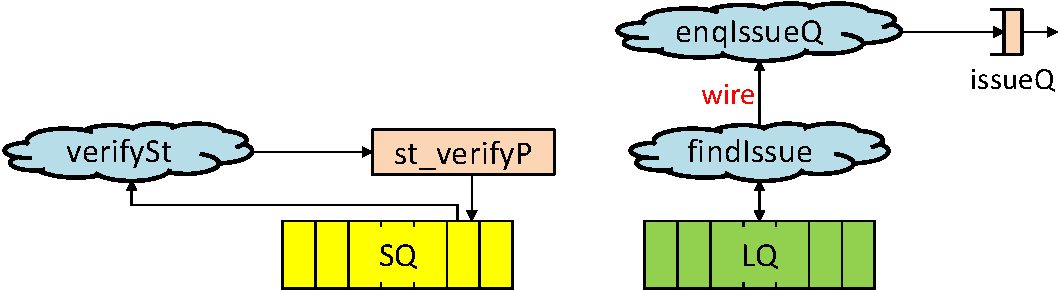
\includegraphics[width=0.7\columnwidth]{fig/lsq_crop.pdf}
    \caption{Internal implementation of LSQ}\label{fig:lsq-impl}
\end{figure}

Figure~\ref{fig:lsq-impl} shows the internal implementation of LSQ.
We use EHRs to store each field of a LQ or SQ entry.
As mentioned earlier, we sequentially verify each SQ entry to ensure that it no longer affect younger loads.
EHR \code{st\_verifyP} points to the SQ entry to be verified next.
Speculative FIFO \code{issueQ} holds loads in LQ that are ready to be issued to execution (i.e., get bypass or access memory).
Method \code{getIssueLd} dequeues this FIFO.
There are three internal rules:
\begin{itemize}
    \item Rule \code{verifySt}: tries to verify that the SQ entry pointed by \code{st\_verifyP} cannot affect younger loads.
    If this is the case, then the rule advances pointer \code{st\_verifyP}, sets field \code{verified} for the SQ entry, and sets field \code{olderStVerified} for applicable LQ entries.
    \item Rule \code{findIssue}: searches LQ for the oldest unissued non-MMIO normal load that is ready to issue.
    The LQ index of the load is recorded in a \emph{wire}.
    \item Rule \code{enqIssue}: reads the value in the wire set by rule \code{findIssue}, and enqueues it into speculative FIFO \code{issueQ}.
\end{itemize}
As we can see, rules \code{findIssue} and \code{enqIssue} should actually be a single rule to ensure atomicity.
However, because \code{issueQ} has the ordering constraint of dequeue before enqueue, the single rule would be ordered after many other rules, and thus, more bypass paths could be introduced.
Since \code{findIssue} performs an associative search, we do not want to introduce bypass paths on it.
Therefore, we split the rule into two, and connect them using a wire.
To make this scheme work, any rule that could affect the LQ entry found by \code{findIssue} must be made conflict with \code{enqIssue}.
Fortunately, only \code{incorrectSpeculation} needs to be conflict with \code{enqIssue}.
It should be noted that since \code{findIssue} does not change any LQ/SQ state, it is fine that \code{enqIssue} fails to fire for whatever reason when \code{findIssue} fires.
However, it is highly desirable to make \code{issueQ} a conflict-free speculative FIFO and put \code{findIssue} and \code{enqIssue} into one rule.

The conflict matrix including the internal rules is (the internal rules are highlighted in red):
\begin{itemize}
    \item \{\code{stqEmpty}, \code{stqFull\_ehrPort0}, \code{ldqFull\_ehrPort0}, \code{noWrongPathLoads}, \code{getOrigBE}, \code{getHit}, \textcolor{red}{\code{findIssue}}\} $<$ \code{deqLd} $<$ \textcolor{red}{\code{verifySt}} $<$ \code{cacheEvict} $<$ \code{updateAddr} $<$ \{\code{getIssueLd}, \code{issueLd}\} $<$ \textcolor{red}{\code{enqIssueQ}} $<$ \{\code{wakeupLdStalledBySB}, \code{deqSt}\} $<$ \code{setAtCommit} $<$ \code{respLd} $<$ \code{updateData} $<$ \{\code{enqLdTag}, \code{enqStTag}\} $<$ \{\code{enqLd}, \code{enqSt}\} $<$ \code{correctSpeculation}
    \item \code{incorrectSpeculation} $<$ \code{correctSpeculation}
    \item \code{incorrectSpeculation} C all others
    \item All others are CF
\end{itemize}
Regarding the problems of \code{issueLd} mentioned before, we have ordered \code{findIssue} before \code{issueLd} and \code{updateAddr}.
That is, the load that calls \code{updateAddr} and \code{issueLd} in the same cycle will not be identified by \code{findIssue}, i.e., no duplicate load issue.

Rules and methods will use the appropriate EHR ports according the conflict matrix.
The only exception is when computing the guard of the \code{enqLd} and \code{enqSt} methods.
The guard is computed using EHR port 0 to avoid bypass from the dequeue methods, and then the computed guard signal is set to a wire checked by the enqueue methods.

\subsubsection{Future Improvement}

\begin{enumerate}
    \item Solve the problem of calling \code{updateAddr} and \code{issueLd} in the same cycle.
    Instead of arbitrating between a newly translated load and a load given by \code{getIssueLd} outside LSQ, we can move this arbitration into LSQ.
    Thus, we always call \code{getIssueLd} outside LSQ to retrieve the load that is ready to issue.
    Then we can hide the problem inside LSQ completely.
    
    \item Merge rules \code{findIssue} and \code{enqIssueQ} into one rule by making \code{issueQ} a conflict-free speculative FIFO.
    
    \item Reconcile fences in case of using a weak memory model is not handled in the optimal way.
    We should put Reconcile fences in LQ and dequeue them earlier than ROB commit time.
\end{enumerate}

\subsubsection{Source Code}
See module \code{mkSplitLSQ} in \code{//procs/lib/SplitLSQ.bsv}.
